%%%%%%%%%%%%%%%%%%%%%%%%%%%%% Define Exam %%%%%%%%%%%%%%%%%%%%%%%%%%%%%%%%%%
\documentclass[addpoints]{exam}
%%%%%%%%%%%%%%%%%%%%%%%%%%%%%%%%%%%%%%%%%%%%%%%%%%%%%%%%%%%%%%%%%%%%%%%%%%%%%%%

%%%%%%%%%%%%%%%%%%%%%%%%%%%%% Using Packages %%%%%%%%%%%%%%%%%%%%%%%%%%%%%%%%%%
\usepackage{amsmath, amssymb, amsthm, amsfonts, geometry, venndiagram, tikz}
\usepackage{graphicx, xcolor, color, wrapfig, parskip, float, tabularx}
\usepackage[breaklinks]{hyperref}
\usepackage{colortbl, caption}
\usepackage{listings, mdframed, subfig, matlab-prettifier, hyperref}
\usepackage{lipsum, bookmark, booktabs, empheq, titlesec, verbatim, subfig, pdfpages, comment}
%%%%%%%%%%%%%%%%%%%%%%%%%%%%%%%%%%%%%%%%%%%%%%%%%%%%%%%%%%%%%%%%%%%%%%%%%%%%%%%
\definecolor{codebackground}{rgb}{0.95,0.95,0.95}
\definecolor{codegray}{rgb}{0.5,0.5,0.5}
\definecolor{codepurple}{rgb}{0.58,0,0.82}
\definecolor{codeblue}{rgb}{0.13,0.29,0.53}
\definecolor{ocre}{RGB}{243,102,25}
\definecolor{mygray}{RGB}{243,243,244}
\definecolor{deepGreen}{RGB}{26,111,0}
\definecolor{shallowGreen}{RGB}{235,255,255}
\definecolor{deepBlue}{RGB}{61,124,222}
\definecolor{shallowBlue}{RGB}{235,249,255}
\definecolor{softgray}{rgb}{0.95, 0.95, 0.95}
\definecolor{codegreen}{rgb}{0,0.6,0}
\definecolor{codegray}{rgb}{0.5,0.5,0.5}
\definecolor{codepurple}{rgb}{0.58,0,0.82}
\definecolor{backcolour}{rgb}{0.95,0.95,0.92}

%Code listing style named "mystyle"
\lstdefinestyle{mystyle}{
  backgroundcolor=\color{backcolour}, commentstyle=\color{codegreen},
  keywordstyle=\color{magenta},
  numberstyle=\tiny\color{codegray},
  stringstyle=\color{codepurple},
  basicstyle=\ttfamily\footnotesize,
  breakatwhitespace=false,         
  breaklines=true,                 
  captionpos=b,                    
  keepspaces=true,                 
  numbers=left,                    
  numbersep=5pt,                  
  showspaces=false,                
  showstringspaces=false,
  showtabs=false,                  
  tabsize=2
}

%"mystyle" code listing set
\lstset{style=mystyle}

\usetikzlibrary{arrows,shapes,positioning,shadows,trees}

%%%%%%%%%%%%%%%%%%%%%%%%%%%%% Header and Footer %%%%%%%%%%%%%%%%%%%%%%%%%%%%%%%%%%
\pagestyle{headandfoot}
\runningheadrule
\runningfootrule
\runningheader{Algorithms: Design and Analysis}{Weekly Challenge 04}{CS 412}
\runningfooter{}{Page \thepage\ of \numpages}{}
\firstpageheader{}{}{}
%%%%%%%%%%%%%%%%%%%%%%%%%%%%%%%%%%%%%%%%%%%%%%%%%%%%%%%%%%%%%%%%%%%%%%%%%%%%%%%

% Other Settings
% \boxedpoints
\printanswers
\qformat{}  %Comment this to number questions, uncomment this to not number questions

\newcommand\union\cup
\newcommand\inter\cap

%%%%%%%%%%%%%%%%%%%%%%%%%%%%%%% Title & Author %%%%%%%%%%%%%%%%%%%%%%%%%%%%%%%%

\title{Algorithms: Design and Analysis - CS 412 \vspace*{-4mm}}
\author{Weekly Challenge 04}
\date{\vspace*{-4mm} Ali Muhammad Asad - aa07190}

% \pgfplotsset{compat=1.18}

%%%%%%%%%%%%%%%%%%%%%%%%%%%%%%%%%%%%%%%%%%%%%%%%%%%%%%%%%%%%%%%%%%%%%%%%%%%%%%%

\begin{document}
\maketitle

% {\small \begin{center} \gradetable[h] \end{center}}

\begin{questions}
  \question[1]
  \textbf{1.}\; (1 point)
  Imagine that you have a 2D grid where each cell contains a color value (see Figure \hyperref[figure1]{1} for an example). Given a start location $(x, y)$, target color, and replacement color, design a recursive algorithm to fill closed regions with a specific color (replacement color). Clearly define a base criterion and analyze the worst-case time complexity of your proposed algorithm/approach.

  Suppose that you have the following array:
  \begin{figure}[h]
    \centering
    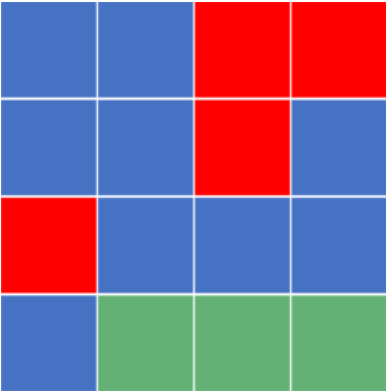
\includegraphics[scale=0.5]{image1.png}
    \caption{Before}
    \label{figure1}
  \end{figure}

  Now, we're given a $start\_position = (0, 0)$ and $new\_color =$ orange. As we can see the color of cell $(0, 0)$ is blue. Therefore, we'll recolor all its connected cells that have the same color to the $new\_color$:

  \begin{figure}[h]
    \centering
    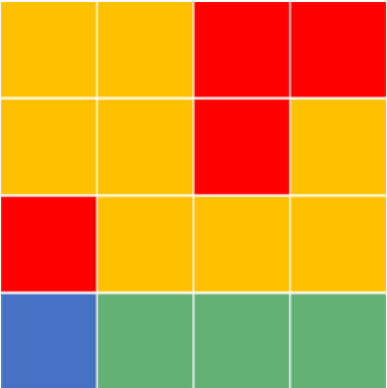
\includegraphics[scale=0.5]{image2.png}
    \caption{After}
  \end{figure}

  \textbf{Input:} start location (row, column), replacement color. \\
  \textbf{Output:} replaces all adjacent cells with the target color with the replacement color. The target color is the original color of the starting location. \\
  \textbf{Moves:} possible moves are up, down, left, right. In addition to up, down, left, and right, you can also add up-right, up-left, down-right, and down-left. \\
  \textbf{Hint:} The algorithm might include recursive calls for each move.

  % \begin{center}
  %     \begin{table}[h!]
  %         \centering
  %         \scalebox{2}{
  %         \begin{tabular}{|c|c|c|c|c|c|l|}
  %             \hline
  %             1 & 1 & 1 & 2 & 2 & 2 & \cellcolor{yellow!25}2 \\
  %             \hline
  %             1 & 1 & 2 & 2 & 2 & 2 & 2 \\
  %             \hline
  %             1 & 1 & 3 & 3 & 3 & 2 & 2 \\
  %             \hline
  %             2 & 1 & 3 & 3 & 3 & 2 & 2 \\
  %             \hline
  %             2 & 1 & 3 & 3 & 3 & 2 & 2 \\
  %             \hline
  %             2 & 1 & 3 & 3 & 3 & 2 & 2 \\
  %             \hline
  %             1 & 1 & 3 & 3 & 3 & 2 & 2 \\
  %             \hline
  %             1 & 1 & 3 & 3 & 3 & 2 & 2 \\
  %             \hline
  %         \end{tabular}}
  %         \caption{The Results}
  %         \label{fig1}
  %     \end{table}
  % \end{center}

  \textbf{Note}: Figure \ref{figure1} is only an example, your algorithm should be valid for any number of colors and any arrangement of the colors.

  \begin{solution}
    We are given a 2D array, where each cell contains a color value. Then our 2D array can be of size $ n \times m $, where $n$ is the rows (number of sub-arrays in our array), and $m$ are the columns (number of elements in each sub-array). Then we need to design an algorithm that replaces the colour of the starting cell with the new color, along with cells sharing the same color that are connected to it. Then for any location $ (i, j) $, or $ (x, y) $ we check the surrounding points $ (x + 1, y), (x - 1, y), (x, y + 1), (x, y - 1) $ if they have the same color as the starting location, and replace its color.

    This can also be thought of as a graph, where each node has some edges connecting to some neighbors, and we have to explore as far as possible before backtracking (in the recursive-based approach), filling the connected nodes with the new color. Then a Depth-First Search (DFS) inspired / based approach can be implemented that works as follows:
    \begin{enumerate}
      \item Start at the given location
      \item Check if the starting row (sr) and starting column (sc) are within the grid boundaries (row and col) to avoid going out of bounds.
      \item Check if the color at the starting position matches the target color. If not, the area doesn't belong to the region, so return.
      \item Fill and Explore: \begin{enumerate}
              \item Change the color of the current cell to the new color.
              \item Recursively explore neighbors by checking all four adjacent neighbors; left, right, up, down, using the new start point as $ (x + 1, y), (x - 1, y), (x, y + 1), (x, y - 1) $.
              \item For each neighbor, repeat steps 1-3, ensuring that only connected regions are filled.
            \end{enumerate}
    \end{enumerate}

    A pseudocode for the above given code is as follows:
    \begin{verbatim}
function fillColor(grid, s_row, s_col, row, col, source, color):
  // Check if the given location is within the grid boundaries
  if s_row < 0 or s_row >= row or s_col < 0 or s_col >= col:
    return
  
  // Check if the color at the position matches the target color
  if grid[s_row][s_col] != source:
    return

  // Mark the cell with the new color
  grid[s_row][s_col] = color

  // Recursively explore the surrounding neighbors
  fillColor(grid, s_row + 1, s_col, row, col, source, color)
  fillColor(grid, s_row - 1, s_col, row, col, source, color)
  fillColor(grid, s_row, s_col + 1, row, col, source, color)
  fillColor(grid, s_row, s_col - 1, row, col, source, color)
end function
\end{verbatim}
    The worst-case time complexity of the above algorithm is the same as the DFS Complexity which is $ O(n \times m) $, where $ n $ is the number of rows, and $ m $ is the number of columns. This is because in the worst case, the algorithm may need to visit each and every cell in the grid, which can happen if the whole grid is filled with a single color. Since we designed our algorithm to only return if the cell does not match the target color, then each cell is only visited once. Hence, the worst time complexity is $ O(n \times m) $.
  \end{solution}

\end{questions}

\end{document}